\documentclass[10pt]{beamer}

\usetheme[progressbar=frametitle]{metropolis}

\usepackage{physics}

\title{Examen parcial 2}
\subtitle{Problemas 10.6 y 14.2}
\author{Jorge Alejandro Rodríguez Aldana}
\institute{Escuela de Ciencias Físicas y Matemáticas - Universidad de San Carlos de Guatemala}
% \titlegraphic{%
%     \includegraphics[width=.5\textwidth]{~/Templates/ecfmLogoColorO.png}\hfill
% }

\titlegraphic{
    \hfill \includegraphics[width = 0.3\textwidth]{Graphics/ecfmLogoColorO.png}
}


\begin{document}

\begin{frame}
    \titlepage
\end{frame} 

\section{Problema 10.6}

\begin{frame}{Problema 10.6}
    \textbf{Efecto de difracción por una unión de Josephson.} 
    Considere una unión de una sección transversal rectangular con un campo magnético $B$ aplicado en el plano de la unión, normal a un borde con ancho $\omega$.
    Digamos que el espesor de la unión es $T$. Asumamos por conveniencia que la diferencia de fase de estos dos superconductores es $\frac{\pi}{2}$ cuando $B=0$.
    Muestre que la corriente $DC$ en la presencia de campo magnético es:

    \begin{equation}
        J\approx J_0\frac{\sin{\omega T B e / \hbar c}}{\omega T B e/\hbar c}
    \end{equation}
\end{frame}

\begin{frame}
    \frametitle{Problema 10.6}

    \begin{figure}
        \centering
        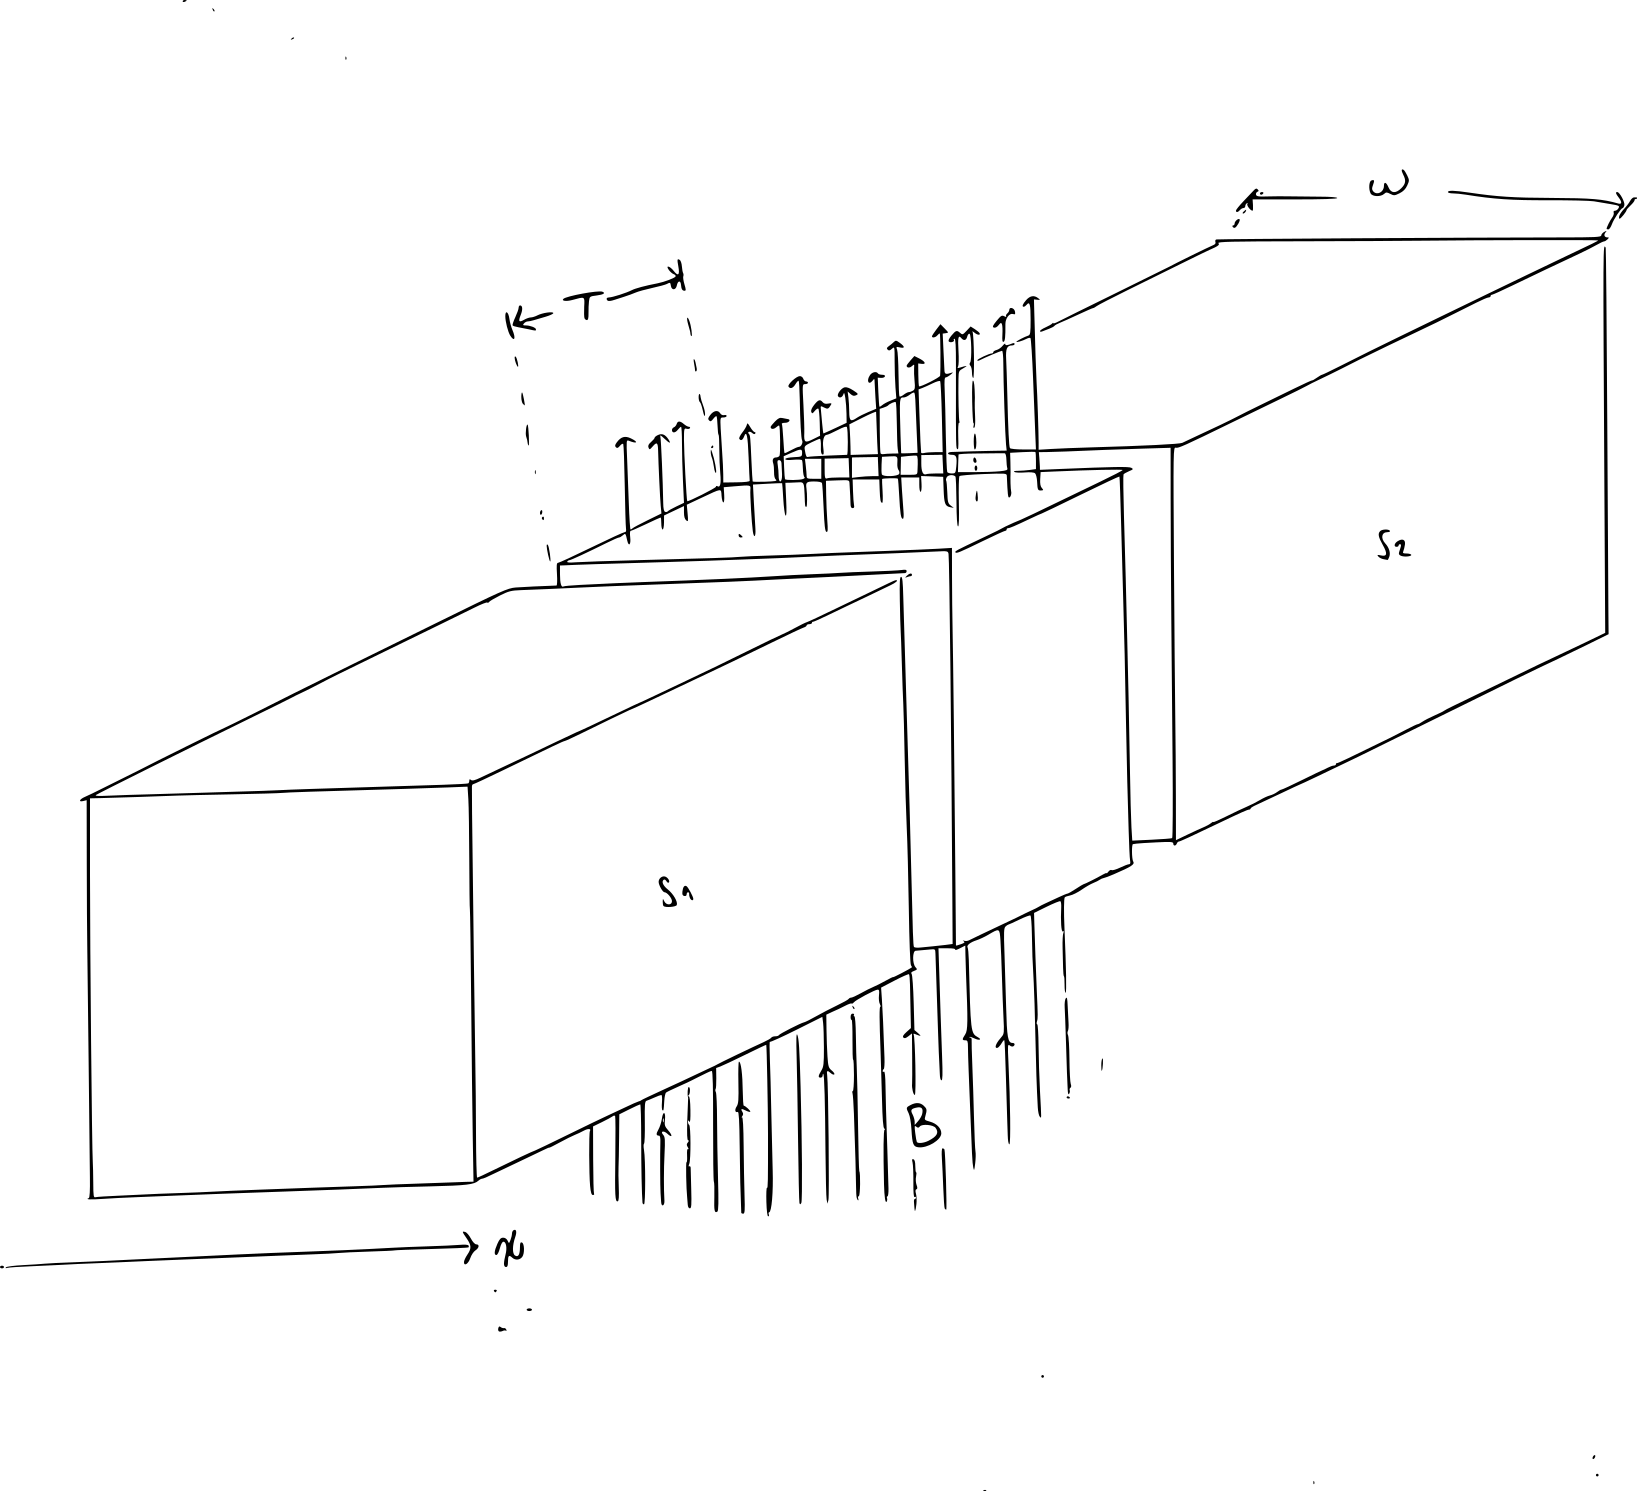
\includegraphics[width=0.8\textwidth]{Graphics/P10-6.png}
        \caption{Planteamiento del sistema}
        \label{fig:P10-6}
    \end{figure}

\end{frame}

\begin{frame}
    \frametitle{Solución - Problema 10.6}

    Calculamos el flujo de campo magnético por un pequeño rectángulo de lados $T$ y $x$. Este es:

    \begin{align*}
        \Phi(x) &= \int_0^x\int_0^T B \dd x \dd T\\
            &= xTB\tag{2}\label{eq:flux}
    \end{align*}

\end{frame}

\begin{frame}
    \frametitle{Solución - Problema 10.6}

    Sabemos que:
    \begin{align*}
        J &= J_o\sin(\delta)\\
        \dd J &= J_o \cos(\delta)\dd \delta
    \end{align*}

    con $\delta =  \frac{e\Phi}{\hbar c} = \frac{exTB}{\hbar c}$

    y $\dd \delta = \frac{eTB}{\hbar c}\dd x$

\end{frame}

\begin{frame}
    \frametitle{Solución - Problema 10.6}

    Ahora, hacemos la siguiente aproximación:

    \begin{align*}
        \frac{exTB}{\hbar c} &= \delta\\
        \frac{eTB}{\hbar c} &=\frac{\delta}{x}\approx\frac{1}{\omega}\\
    \end{align*}

\end{frame}

\begin{frame}
    \frametitle{Solución - Problema 10.6}

    \begin{align*}
        \dd J &\approx J_0 \cos\left(\frac{xeTB}{\hbar c}\right)\frac{1}{\omega}\dd x\\
        J & \approx \int_0^\omega \cos\left(\frac{xeTB}{\hbar c}\right)\frac{1}{\omega}\dd x\\
        J &\approx J_0\frac{\sin{\omega T B e / \hbar c}}{\omega T B e/\hbar c}
    \end{align*}

\end{frame}

\section{Problema 14.2}

\begin{frame}
    \frametitle{Problema 14.2}

    \textbf{Plasmones de interferencia.} Consideramos un plano $z=0$ entre un metal $1$ a $z>0$ y un metal $2$ a $z<0$. El metal $1$ tiene una frecuencia de plasmón $\omega_{p1}$; el metal $2$ de $\omega_{p2}$. El dieléctrico entre esos dos metales es de gases de electrones libres. Muestre que los plasmones de superficie asociados con la interfaz tienen una frecuencia de:

    \begin{align*}
        \omega = \left[\frac{1}{2}\left(\omega_{p1}^2+\omega_{p2}^2\right)\right]^{1/2}
    \end{align*}

\end{frame}

\begin{frame}
    \frametitle{Solución - Problema 14.2}

    Partimos de las siguientes ecuaciones del libro:

    \begin{align*}
        \epsilon(\omega) = 1-\frac{\omega_p^2}{\omega^2} \tag{10}
    \end{align*}

    \begin{align*}
        \omega_s^2 = \frac{1}{2}\omega_p^2 \tag{71}
    \end{align*}

    Con $\omega_s$ la frecuencia de una superficie de un plasma semi infinito en el lado positivo de un plano $z=0$.

\end{frame}

\begin{frame}
    \frametitle{Solución - Problema 14.2}

    \textbf{Proposición:}
    \begin{equation*}
        \epsilon_1(\omega) = -1
    \end{equation*}

    En la superficie de plasma.

    \textbf{Demostración:}

    Partiendo de las ecuaciones anteriores, en la superficie $\omega = \omega_s$.

    \begin{equation*}
        \epsilon_n(\omega) = 1-\frac{\omega_{pn}^2}{\omega_s^2} = 1-\frac{\omega_{pn}^2}{\frac{1}{2}\omega_{pn}^2} = -1
    \end{equation*}

    \qed

    Análogamente, para la frecuencia en la superficie de un plasma semi infinito en el lado negativo de un plano $z=0$:

    \begin{equation*}
        \epsilon_2(\omega) = 1
    \end{equation*}

\end{frame}

\begin{frame}
    \frametitle{Solución - Problema 14.2}

    Entonces, partiendo de esto tenemos:

    \begin{align*}
        \epsilon_1(\omega) &= -\epsilon_2(\omega)\\
        1-\frac{\omega_{p1}^2}{\omega^2} &= -1+\frac{\omega_{p2}^2}{\omega^2}\\
        2 &= \frac{\omega_{p1}^2}{\omega^2} +\frac{\omega_{p2}^2}{\omega^2}\\
        \omega^2 &= \frac{1}{2}\left(\omega_{p1}^2+\omega_{p2}^2\right)\\
        \omega &= \left[\frac{1}{2}\left(\omega_{p1}^2+\omega_{p2}^2\right)\right]^{1/2}
    \end{align*}

    \qed

\end{frame}

\end{document}